\chapter{Các thành phần trong Ruby on Rails}
Chương này trình bày chi tiết về các thành phần chính trong framework Ruby on Rails.


\section{Các thành phần chính trong Rails}
Các thành chính trong Rails gồm : Model, View, Controller và Routing, hình ~\ref{fig:4c} chỉ ra vị trí của 4 thành phần trong Rails. Các thành phần tương tác, quan hệ chặt chẽ với nhau. Việc cấu hình để các thành phần này hoạt động với nhau được Rails đơn giản hóa đi rất nhiều bằng cách cung cấp quy ước cấu hình, đúng theo triết lý Convention over Configuration. Bên cạnh đó Rails cũng cung cấp các lệnh tương tác với shell để tạo ra các thành phần trên một cách thuận lợi và đúng quy chuẩn nhất. 
\begin{figure}
	\centering
		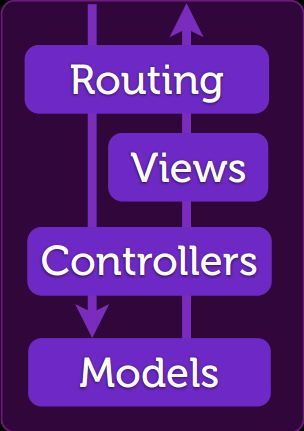
\includegraphics[width=5cm, height=7cm]{image/4c.JPG}
	\caption{4 thành phần chính trong Rails}
	\label{fig:4c}
\end{figure}

\section{Model trong Rails}
Model là một thành phần được cho là quan trọng nhất trong các ứng dụng Ruby on Rails, Rails hỗ trợ rất nhiều các thành phần để việc làm việc với Model trở lên dễ dàng và tiện lợi, các thành phần hỗ trợ cho Model được đặt trong một module là Active Record. Các model trong Rails kế thừa lớp Base từ module ActiveRecord. Các model được đặt trong thư mục model trong thư mục app của 1 project Rails.

\subsection{Ánh xạ model với các bảng dữ liệu}
Một bảng dữ liệu trong cơ sở dữ liệu quan hệ được biểu diện bởi một model. Các model trong Rails được cài đặt theo mẫu thiết kế Active Record giúp việc thao tác với các bảng dữ liệu trở lên dễ dàng thông qua các method được cung cấp sẵn, gồm các thao tác Creat, Read, Update, Delete - CRUD.
Model được tạo tự động bằng câu lệnh "rails generate model". Đoạn code ~\ref{model1} chỉ ra các tạo một model từ một câu lệnh, và thao tác với cơ sở dữ liệu

\begin{lstlisting}[
language=Ruby,
label=model1,
inputencoding=utf8,
caption=Model class trong Rails
]

# rails generate model User name:string phone:string
# A model class
class User < ActiveRecord::Base
end

# CRUD with model
# Create and store a model into database
User.create(:name => "user 1")

# Get a model from database by id
user = User.find(1)

# Update a model
user.update_attributes(:name => "USER 1")

# Delete a User by id
User.destroy(1) 

\end{lstlisting}

\subsection{Data migrations}
Data migrations là một cách để tạo, thay đổi các bảng dữ liệu trong Rails, thay vì phải viết các lệnh SQL để tạo cấu trúc của các bảng dữ liệu, migrations là các Ruby class, ở mức trừu tượng cao hơn, tọa thuận lợi cho việc viết mã cũng như dễ đọc và bảo trì và quản lý. Migrations độc lập với cơ sử dữ liệu vật lý sử dụng bên dưới, tùy thuộc vào hệ quản trị cơ sở dữ liệu sử dụng mà migrations được dịch thành các mã SQL phù hợp. Bên cạnh đó migration cũng là cho việc quản lý các phiên bản của cơ sở dữ liệu một cách thuận lợi bằng việc đánh phiên bản cho mỗi lần thay đổi cơ sở dữ liệu sử dụng migration, từ đó có thể chuyển đổi các phiên bản tùy ý. \newline

Mỗi model được tạo ra bằng lệnh của Rails, thì 1 class migration được tạo ra tương ứng với model đó. Các migration class kế thừa class Migration từ model ActiveRecord. Để tạo bảng dữ liệu từ migration class dùng lệnh rake db:migrate. Đoạn code ~\ref{model2} mô tả một migration class.
 \begin{lstlisting}[
language=Ruby,
label=model2,
inputencoding=utf8,
caption=Migration class trong Rails
]
# Migration class for creating users table
# Generated from User's generation
class CreateUsers < ActiveRecord::Migration
    def change  
       create_table :users do |t|
          t.string :name
          t.string :phone
          t.timestamps
       end
    end
end
\end{lstlisting}


\subsection{Quan hệ giữa các model}
Các bảng dữ liệu trong hệ cơ sở dữ liệu quan hệ cũng có các quan hệ với nhau như 1-nhiều, 1-1, nhiều-nhiều, các model biểu diễn các bảng dữ liệu nên giữa các model cũng có những quan hệ này.
Rails cung cấp một số method để việc tạo các quan hệ này giữa các model trở lên dễ dàng, chỉ phải thêm các method cho các quan hệ tương ứng và bên trong phần định nghĩa của các model class thì các quan hệ được thiết lập. Việc này giúp cho việc lập trình trở lên cực kì thuận tiện và dễ dàng, thay vì phải tạo các file cấu hình rất dài, đối với các framework khác.
 

Ví dụ tạo quan hệ giữa 2 model Order và Customer, một Order thuộc về 1 Customer được biểu diễn bằng method \texttt{belongs\textunderscore to}, Customer có nhiều Order, được biểu diễn bằng method \texttt{has\textunderscore many}. Lúc này order có thể biết được customer và customer có thể quản lý được các order của mình đã đặt.
Hình~\ref{fig:belongs_to} và~\ref{fig:has_many} và mô tả việc tạo quan hệ giữa 2 model Order và Customer.
\begin{figure}
	\centering
		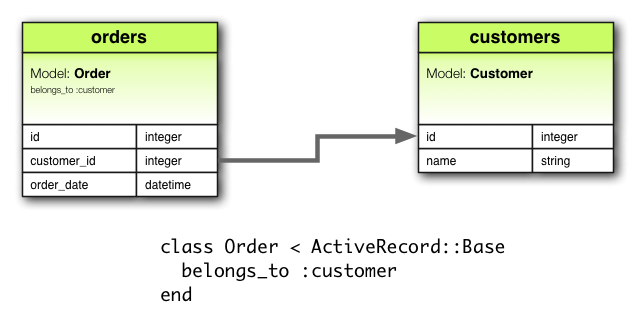
\includegraphics[width=14cm, height=8cm]{image/belongs_to.png}
	\caption{1 Order thuộc về 1 Customer}
	\label{fig:belongs_to}
\end{figure}
\begin{figure}
	\centering
		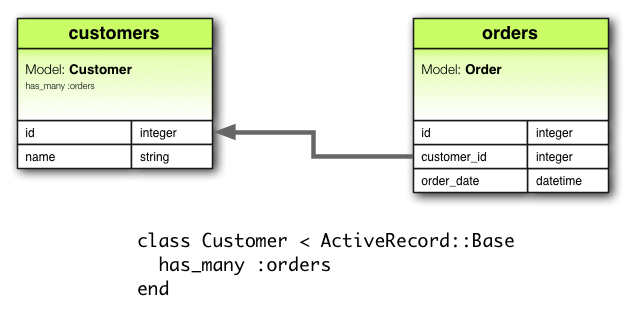
\includegraphics[width=14cm, height=8cm]{image/has_many.png}
	\caption{1 Customer có nhiều Order}
	\label{fig:has_many}
\end{figure}


\section{Controller trong Rails}
Controller là thành phần điều phối tất các thành phần còn lại như Model và View. Controller trong Rails kế thừa lớp ActionController::Base, các controller được đặt trong thư mục controller của thư mục app, giúp việc quản lý trở lên thuận tiện.
Một controller có nhiều các method, mỗi phương thức tương ứng với một action sẽ thực hiện bởi các request từ người dùng. Rails cũng cung cấp một câu lệnh chuẩn để tạo controller. Đoạn code~\ref{controller} chỉ ra các tạo một model trong Rails.

\begin{lstlisting}[
language=Ruby,
label=controller,
inputencoding=utf8,
caption=Controller trong Rails
]
# rails generate controller welcome index
# A controller with a method and view both named index 
class WelcomeController < ApplicationController
    # GET welcome/index
    def index
    end
end

\end{lstlisting}

Mỗi method trong conttroller sẽ được gọi tới bằng môt HTTP request, và mỗi method sẽ được gắn với một request xác định được quy định trong thành phần định tính của ứng dụng Rails.

\section{View trong Rails}
View là thành phần dùng để hiển thị dữ liệu từ model được cung cấp bởi controller, view là thành phần mà các triết lý của Rails được thể hiện rõ nhất, bằng việc hỗ trợ tự động sinh mã sử dụng method render.
Mỗi view được biểu diễn bởi một file có phần mở rộng .html.erb và tương ứng với một method trong controller tương ứng, tất cả các view của một controller được đặt trong một thư mục có tên là controller đó nằm trong thư mục app/view, hình ~\ref{fig:d} là cấu trúc của một project Rails chuẩn.
\begin{figure}
	\centering
		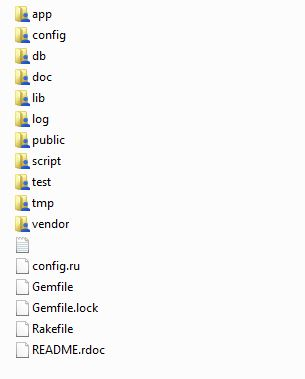
\includegraphics{image/d.JPG}
	\caption{Cấu trúc 1 project Rails}
	\label{fig:d}
\end{figure}

Thư mục app là thư mục chứa các controller, view, model. Thư mục db chứa các thành phần về cơ sở dữ liệu, thư mục test chứa các thành phần để test ứng dụng.

View trong rails được tạo theo các mẫu có sẵn hay gọi là các template. Ví dụ có thể sinh tự động các view từ model bằng cách dùng câu lệnh rails g scaffold, đoạn code ~\ref{view} mô tả việc tạo các view cho một model.
 
\begin{lstlisting}[
language=Ruby,
label=view,
inputencoding=utf8,
caption=Tạo form tự động cho việc tạo model post
]
# rails generate scaffold post 
# name:string title:string content:text
<%= form_for(@post) do |f| %>
  <div class="field">
    <%= f.label :name %><br />
    <%= f.text_field :name %>
  </div>
  <div class="field">
    <%= f.label :title %><br />
    <%= f.text_field :title %>
  </div>
  <div class="field">
    <%= f.label :content %><br />
    <%= f.text_area :content %>
  </div>
  <div class="actions">
    <%= f.submit %>
  </div>
<% end %>

\end{lstlisting}

\section{Routing trong Rails}
Routing có nhiệm vụ đưa các request từ người dùng tới các method trong controller một cách phù hợp.
Mỗi HTTP request trước khi được gửi tới các method trong controller được xử lý, sẽ được kiểm tra trong bảng định tuyến của thành phần routing, nếu request đó tương ứng với một method trong controller nào đó, thì method đó sẽ được gọi. Hình ~\ref{fig:routing} là bảng định tuyến của một controller là posts với các method tương ứng trong bảng.
\begin{figure}
	\centering
		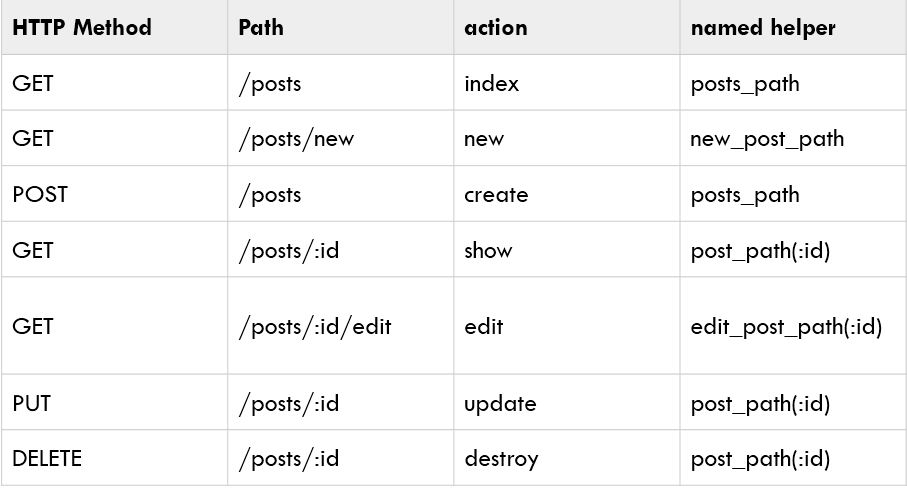
\includegraphics[width=14cm, height=10cm]{image/routing.JPG}
	\caption{Bảng định tính của controller posts}
	\label{fig:routing}
\end{figure}

Việc định tuyến được quy định trong file routes.rb trong thư mục config, Rails cung cấp một các dễ dàng để tạo một bảng định tuyến như hình~\ref{fig:routing} bằng cách thêm dòng lệnh resources :posts trong file routes.rb, để xem tất cả các định tuyến trong 1 ứng dụng sử dụng câu lệnh rake routes.
\newline

{\bf Tổng kết}\newline Các thành phần trong Ruby on Rails đều được thiết kế giúp việc xây dựng ứng dụng trở lên nhanh gọn và thuận tiện nhất, mang đúng tư tưởng của phương pháp phát triển phần mềm agile, giúp cho người lập trình tăng năng suất và sự hài lòng.

